\documentclass{memo}
\usepackage{graphicx}
\usepackage{hyperref}

\memoto{Dr. Simoni}
\memofrom{Kyle Daruwalla and Sunil Rao}
\memosubject{Milestone 1 Update}
\memodate{\today}

\begin{document}

\maketitle

\section{Overview}
Our group is focused on optimizing for power. To accomplish this task, we have investigated low power designs for the adder and comparator units within the overall architecture (note that the multiplier unit will also see a power reduction as it contains several adders). Additionally, we considered generic power reduction strategies like clock gating. Furthermore, we would like to reduce the supply voltage for simpler structures by using transistors with lower threshold voltages.


\section{Design Methodologies}

\subsection{Clock Gating}
Clock gating is a typical method to ``turn-off'' portions of the design that are not being used. As a result, clock gating will help reduce our dynamic power consumption.

\subsection{Lower Threshold Voltages}
For simpler structures without complex datapaths, it is possible to use transistors with lower threshold voltages without affecting the operation. In order to achieve this strategy, we will need to investigate if the technology library available to us offers FETs with varying threshold voltages. Using a lower threshold voltage will allow us to use a lower supply voltage. This strategy for reducing power is particularly useful because of the relationship between supply voltage and power consumption: $$P = \alpha f_{clk} C_L V_{DD}^2$$ where $P$ is the power consumed, $\alpha$ is the activity factor, $f_{clk}$ is the clock frequency, $C_L$ is the load capacitance, and $V_{DD}$ is the supply voltage. So, reducing the supply voltage by a factor will reduce the power quadratically.

\subsection{Low Power Comparator}
We will use a low power comparator design presented in ``CMOS Comparators for High-Speed and Low-Power Applications'' \cite{menendez}. The benefit of this topology is that every bit of the comparison is a separate stage, and each stage is pre-charged high while the clock is low. Thus, when the clock goes high, the output will only have a path to discharge to ground if the input $A > B$. The end result is a comparator that has fewer switching signals and a lower dynamic power consumption. The design can be seen in Figure \ref{fig:low-power-comparator}.
\begin{figure}[h]
    \centering
    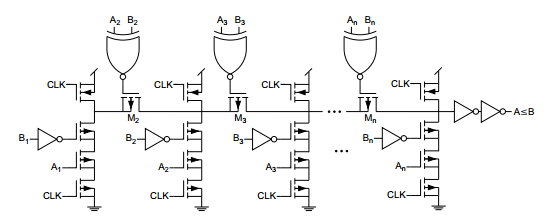
\includegraphics{low-power-comparator.png}
    \caption{Low power comparator circuit \cite{menendez}}
    \label{fig:low-power-comparator}
\end{figure}

\subsection{Static Energy Recovery Full (SERF) Adder }
We will use a SERF adder in order to minimize power consumption in the multiplier and adder unit. The SERF adder minimizes power consumption by eliminating a direct path to ground. In a traditional logic design, the charge at the output stored in the load capacitance is discharged to ground during a high to low transition. In this design, because there is no ground, it won't discharge the load capacitance. Instead, the charge on the load capacitance is used to bias other transistors in the circuit. This reduces power consumption as you have less current flowing in the circuit at logic transitions. The circuit design can be see in Figure \ref{fig:serf-adder-design}.
\begin{figure}[h]
    \centering
    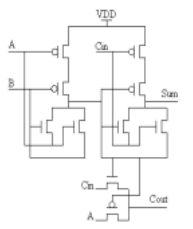
\includegraphics{serf-adder.png}
    \caption{SERF adder circuit \cite{shalem}}
    \label{fig:serf-adder-design}
\end{figure}

\subsection{Booth Multiplier}
We will use Booth multiplier for the multiplier unit. Since this topology is designed to reduce the number of partial products (and thus the amount of logic), it is inherently low power. In Figure \ref{fig:booth-multiplier}, a standard booth multiplier block diagram is shown. To reduce the power consumption even further, we will replace the carry-lookahead (CLA) adders with SERF adders.
\begin{figure}[h]
    \centering
    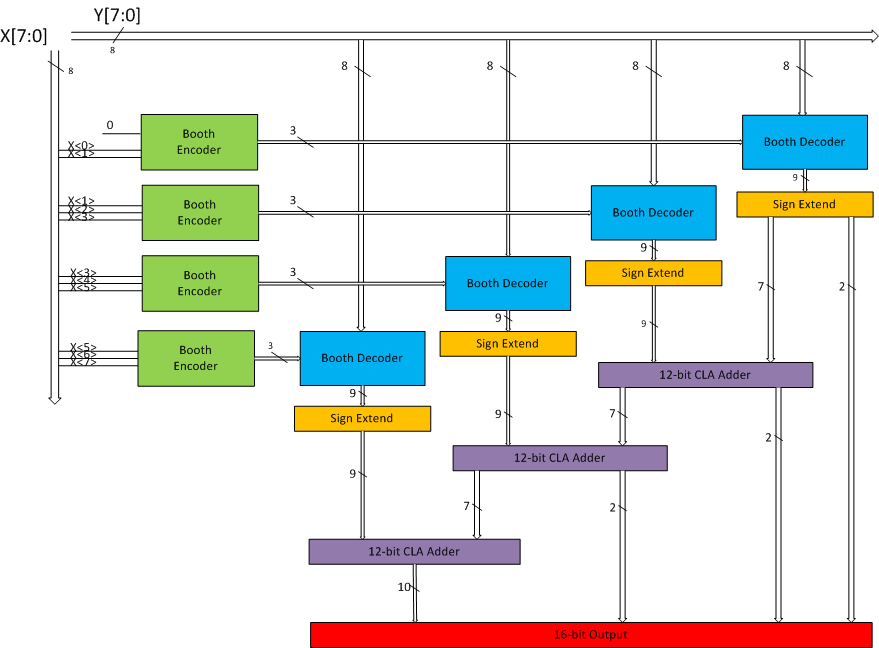
\includegraphics[scale=0.5]{booth-multiplier.png}
    \caption{Standard 8-bit Booth Multiplier \cite{dangelo}}
    \label{fig:booth-multiplier}
\end{figure}

\newpage

\begin{thebibliography}{9}
    \bibitem{dangelo}
    R. D'Angelo and S. Smith. \textit{Modified Booth Multiplier}. Introduction to VLSI Design, EE 103, 2011. Web. 13 April 2016. \\ \url{http://www.eecs.tufts.edu/~rjdang/index2.html}
    \bibitem{menendez}
    E. R. Menendez, D. K. Maduike, R. Garg, and S. P. Khatri. \textit{CMOS Comparators for High-Speed and Low-Power Applications}. International Conference on Computer Design, October 2007, pp. 76-81. \\ \url{https://pdfs.semanticscholar.org/bffe/2300176526562d02743ed01832fa2b22aa82.pdf}
    \bibitem{shalem}
    R. Shalem, E. John, L.K. John. \textit{A Novel Low Power Energy Recovery Full Adder Cell}. Great Lakes Symposium on VLSI,  1999, pp. 380. \\ \url{https://lca.ece.utexas.edu/pubs/roy.pdf}
\end{thebibliography}

\end{document}